% Prämabel
\documentclass[11pt,a4paper]{article}

% Codage
\usepackage[utf8]{inputenc}
\usepackage[T1]{fontenc}
\usepackage{siunitx}
\usepackage{indentfirst}

% Langue
\usepackage[english]{babel}

% Supplément
\usepackage{amsmath,amsfonts,amssymb}
\usepackage{verbatim} % pour faire des commentaires avec \begin{comment}...
\usepackage{float} % pour positioner un image exacetement où on veut
\usepackage
  [separate-uncertainty = true,
  multi-part-units = repeat]
  {siunitx} % Exemple \SI{0}{\kg \cdot \m^{-3}}

% Images
\usepackage[pdftex]{graphicx}
\usepackage{graphics}
\usepackage{subcaption} % pour positioner des figures côte à côte
\usepackage{wrapfig}

% pour l'inclusion de liens dans le document 
\usepackage[colorlinks,bookmarks=false,linkcolor=blue,urlcolor=blue]{hyperref}


% la mise en page
\usepackage{geometry}
\paperheight=297mm
\paperwidth=210mm

\pagestyle{plain}



% nouvelles commandes LaTeX, utilis\'ees comme abreviations utiles
\newcommand{\mail}[1]{{\href{mailto:#1}{#1}}}
\newcommand{\ftplink}[1]{{\href{ftp://#1}{#1}}}

%%%%%%%%%%%%%%%%%%%%%%%%%%%%%%%%%%%%%%%%%%%%%%%%%%%%%%%%
\begin{document}


% Le titre, l'auteur et la date
\title{Numerical Exercise \#2}
\author{Caspar Gutsche\\  % \\ pour fin de ligne
}
\date{\today}
\maketitle
%%%%%%%%%%%%%%%%%%%%%%%%%%%%%%%%%%%%%%%%%%%%%%%%%%%%%%%%



\newpage
\section{Question \#1}
Numerical solution for the bare system \\
keff (scientific format with 5 significant digits): k = 0.97511 \\
net current at the core boundary (scientific format with 5 significant digits): $J = \frac{\phi_{2}-\phi_{1}}{dx}= 0.07106$ \\
\begin{figure}[h]
	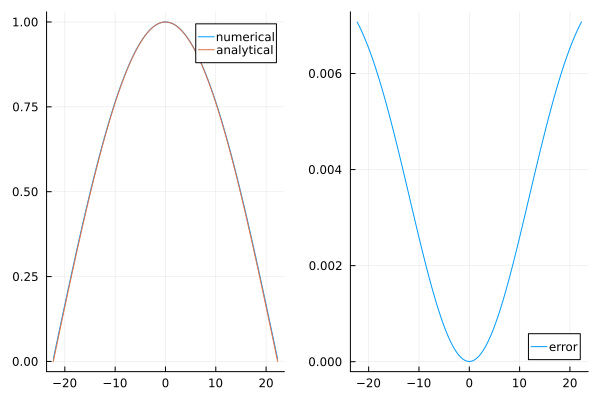
\includegraphics[width=7cm]{../figs/ex2/bare.png}
	\centering
	\caption{Flux in the bare reactor for a mesh size of 0.1 cm and Distance between numerical and algebraic solutions at each mesh point for a mesh size of 0.1 cm.}
\end{figure}

\section{Question \#2}
% \begin{figure}[h]
% 	%\includegraphics[width=7cm]{IMage/SSjeff33_Al_geom1.png}
% 	\centering
% 	\caption{Distance between the solutions at each mesh point for a mesh size of 0.1 cm.}
% \end{figure}
Analytical solution for the bare system\\
For the bare reactor the Equation becomes
$$
\frac{d^2 \phi}{d z^2}+B_m^2 \phi=0
$$
where $B_{m}$ is the material Buckling. 
It is solved by $\phi(z)=A \cos (B z)+C \sin (B z)$. Due to the symmetric boundary conditions of the problem, we know that $C=0$. The geometric buckling is $B^2=\left(\frac{\pi}{H+2 d}\right)^2$.
A steady state is reached, when the material Buckling is equal to the numerical buckling, in this case, $k_{eff}$ can be calculated by
$$
k_{\mathrm{eff}}=\frac{k_{\infty}}{1+L^2 B^2}
$$

keff (scientific format with 5 significant digits):  0.97785\\
net current at the core boundary (scientific format with 5 significant digits): 0.1607 (left and right)\\

\section{Question \#3}
Numerical solution for the reflected system \\
keff (scientific format with 5 significant digits):1.14649\\
net current at the core boundary (scientific format with 5 significant digits): 0.03285\\
\begin{figure}[h]
	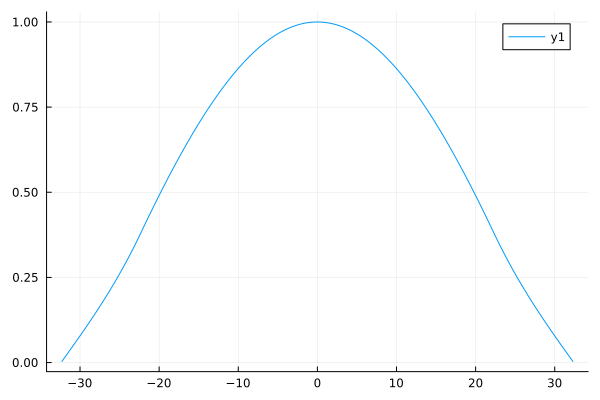
\includegraphics[width=7cm]{../figs/ex2/reflector.png}
	\centering
	\caption{Flux in the reflected reactor for a mesh size of 0.1 cm.}
\end{figure}

%%%%%%%






\end{document}
